\section{The shot-noise programme}
\label{sec:shots}

\Cref{sec:noise} found that, at today's published error rates, what limits a hardware
demonstration of these networks is not gate error but the number of measurements.  Two
mechanisms were identified: a thresholded controller whose decisions sit close to its threshold
flips at a rate set by $\Phi(-2\delta\sqrt N)$; and a histogram loss estimated from $N$ shots is
biased upward by $(K-1)/(2\,\Pout\,N)$ and discards the half of the shots in which the output
did not fire.  Six remedies were proposed; this section reports the three we implemented and
tested (\cref{tab:shots-summary}).  All runs are noiseless state-vector simulations plus
sampling, minutes each.

\begin{table}[t]
\centering\small
\caption{The shot-noise programme: what was tried and what came out.  Items 4--6
(joint-distribution loss or amplitude amplification to use all shots; bias-corrected KL
estimators; amplitude estimation) are designed but not implemented.}
\label{tab:shots-summary}
\begin{tabularx}{\textwidth}{@{}l X X@{}}
\toprule
Remedy & Mechanism & Outcome \\
\midrule
1. Margin-aware training & add a penalty for frames whose margin $\delta$ is below $m=0.1$ &
\textbf{negative}: margins of this network barely move; play under shot noise gets worse \\
2. Common random numbers & evaluate the two finite-difference probes on the same measurement
randomness (maximal coupling) & derivative variance $\div 3$ at our reproduction's step ($c=0.2$), $\div 12$--$22$
at small steps; sampled training improves at $N\le 4\,000$ but stays $10\times$ above the
exact-probability result, consistent with the bias of the loss itself \\
3. Sequential decisions & Wald's sequential test on the sign of $\Pout-\tfrac12$ per frame &
\textbf{positive}: $100\,\%$ perfect games at about $2\,200$ shots/frame, $4.6\times$ fewer than
the fixed budget that achieves the same \\
\bottomrule
\end{tabularx}
\end{table}

\subsection{Margin-aware training (negative result)}
\label{sec:margin}

The idea: if the controller could be trained so that every frame it visits has
$\delta\ge 0.1$ instead of the median $0.019$, the shots needed per frame would fall by
$(0.1/0.019)^2\approx 25\times$, at no cost on a noiseless simulator.  We added to the training
objective a penalty of $w\times 0.01\times\max(0, 1-\delta/m)$ per played frame --- a fraction
$w<1$ of the $0.01$ reward for surviving that frame, so that surviving a frame is always worth more
than dying confidently --- and fine-tuned the trained controller for 25 sweeps with $m = 0.1$
and $w\in\{0.25, 0.5, 1\}$ (run \run{flappy\_shots/20260821T084601Z}).  A first attempt with a
\emph{mean} hinge of weight 20, trained from scratch, had collapsed to a policy that died in 30
frames with perfectly confident decisions (run \run{…T075048Z}): any penalty that can outweigh
the per-frame reward selects for dying early, which is why the per-frame form is necessary.

\Cref{fig:flappy-shots} (left) shows the outcome: the margin quantiles hardly move (median
$0.019\to0.021$--$0.024$, tenth percentile $0.004\to0.006$).  All three fine-tuned controllers
still play perfectly on exact probabilities, but under shot noise they play \emph{worse} than the
original at $w\ge 0.5$ ($50\,\%$ and $80\,\%$ perfect games at $10\,000$ shots against
$100\,\%$).  The explanation is in \cref{fig:flappy-policy}: the activation is a smooth surface
over the two observations, and the near-boundary frames are those in which the bird hovers at
the boundary --- a property of the game's dynamics, not of the surface's steepness.  Penalising
them moves the boundary rather than steepening it, and a moved boundary is a less stable
controller.  A 17-parameter network has no spare capacity to steepen its surface.  We record
the remedy as not working for this network.

\begin{figure}[t]
\centering
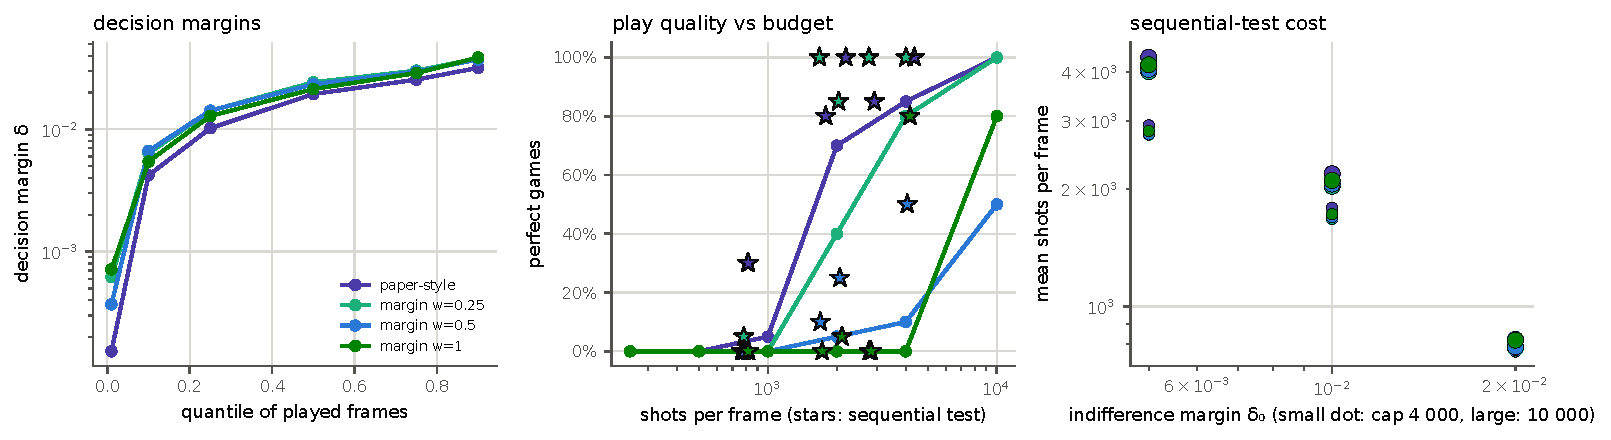
\includegraphics[width=\textwidth]{fig_flappy_shots_programme}
\caption{Flappy under shot noise, remedies 1 and 3.  Left: decision-margin quantiles of the
frames played by the original and the three margin-aware controllers.  Middle: perfect games
against shots per frame for a fixed budget (lines) and for the sequential test (stars, at the
mean shots it actually spent).  Right: mean shots per frame of the sequential test against its
indifference margin $\delta_0$.  Run \run{flappy\_shots/20260821T084601Z}.}
\label{fig:flappy-shots}
\end{figure}

\subsection{Common random numbers for the finite-difference optimiser}
\label{sec:crn}

\paragraph{Mechanism.}
The paper's optimiser estimates a slope as $(f(x+c)-f(x-c))/2c$.  If each probe is estimated
from $N$ independent shots with variance $\sigma^2$, the slope has variance $\sigma^2/2c^2$ ---
at our reproduction's $c=0.2$ that is $12.5\sigma^2$, which is why finite differences on a
sampling backend stall.  If the two probes are instead computed from the \emph{same} random draws, the
noise largely cancels.  The standard way (feeding the same uniform random numbers to the inverse
cumulative distribution of both probes) turned out to give only a $1.3\times$ reduction here,
because a parameter change moves probability between distant bit strings and so shifts every
later bin boundary.  What works is the \emph{maximal coupling} \cite{lindvall}: sample the first
probe, then for the second keep each shot's outcome $i$ with probability
$\min(1, p_{\mathrm{new}}(i)/p_{\mathrm{ref}}(i))$ and redraw it otherwise from the excess
$(p_{\mathrm{new}}-p_{\mathrm{ref}})_+$.  The second sample has exactly the right distribution,
and only $N\cdot\TV(p_{\mathrm{new}},p_{\mathrm{ref}})$ shots change --- the fewest any coupling
can achieve.  Since $\TV\propto c$, the difference of the two estimates has variance $O(c/N)$ and
the slope, after division by $2c$, has variance $O(1/(cN))$ instead of $O(1/(c^2N))$: a gain of
order $1/c$.  Coupling reduces the variance of the slope; it does not remove the bias of a
non-linear loss such as the plug-in KL.  On hardware the analogue is to interleave the $\pm c$ circuits in one job so they
share the same drift.

\paragraph{Measurement.}
\Cref{fig:crn} measures the variance of one slope of the bit-count loss at $400$ shots per
probe: the reduction is $\times 2$--$3$ at $c=0.2$--$0.4$ and $\times 22$--$29$ at $c=0.025$--$0.05$,
as the $1/c$ scaling predicts, and both estimates are unbiased for the exact slope.
\Cref{fig:sampled-training} then trains the 11-qubit bit-count network with our reproduction's
schedule (the paper publishes none) on a sampling backend (run \run{bitcount\_shots/20260821T084558Z}): at $N=1\,000$
shots per evaluation the exact KL after 20 sweeps improves from $0.080$ to $0.059$ with common
random numbers, at $4\,000$ from $0.050$ to $0.014$, and at $16\,000$ the two are within the
seed-to-seed spread ($0.029$ vs $0.033$).  All of them remain an order of magnitude above the
exact-probability result ($0.0009$).  The right panel suggests why: the \emph{loss} is the plug-in
KL of a 32-bin histogram from about $N/2$ usable shots, biased by $31.8/N$, and the reached KL
tracks one to three times that bias.  This is consistent with the estimator, not the optimiser,
being what now limits sampled training, but three seeds (one of which stalls at $0.014$ even on
exact probabilities) cannot separate the two; a bias-corrected or joint loss under paired
initialisations is the test, and it has not been run.  Our step schedule ($c_0 = 0.2$ decaying
only to $0.15$ over 20 sweeps) also keeps the optimiser in the regime where the reduction is
smallest.

\begin{figure}[t]
\centering
\begin{minipage}[t]{0.47\textwidth}\centering
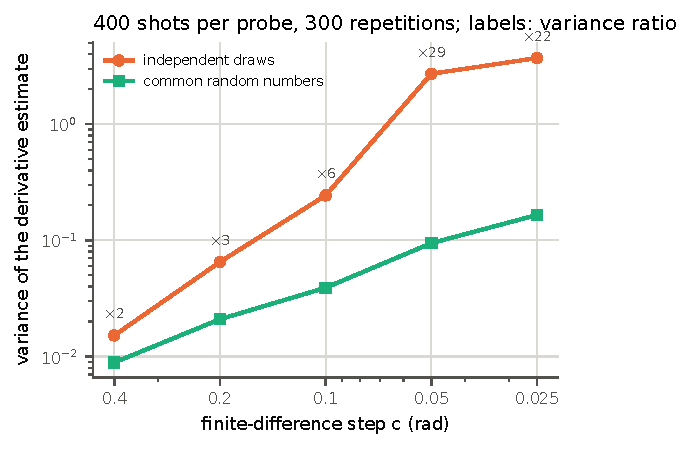
\includegraphics[width=\textwidth]{fig_crn_variance}
\caption{Variance of the finite-difference slope of the bit-count loss at 400 shots per
probe, with independent draws and with maximally coupled draws; labels give the ratio.}
\label{fig:crn}
\end{minipage}\hfill
\begin{minipage}[t]{0.5\textwidth}\centering
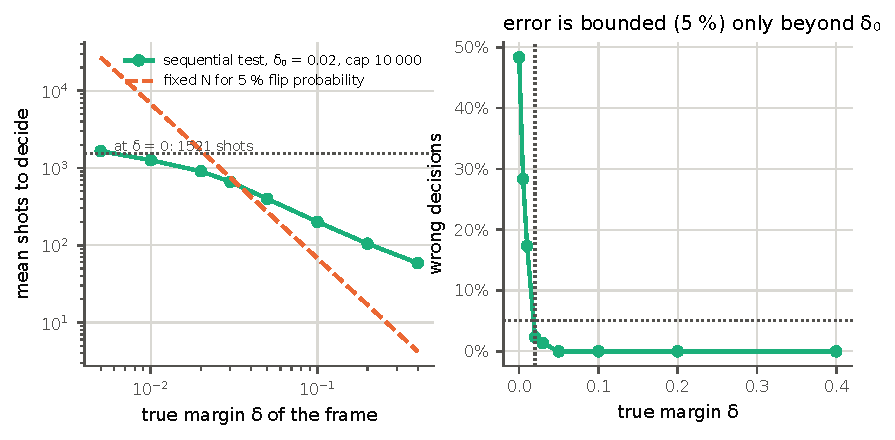
\includegraphics[width=\textwidth]{fig_sprt_cost}
\caption{The sequential test ($\delta_0=0.02$, $5\,\%$ error bounds, cap $10\,000$): mean
shots to decide a frame against its true margin (left), and its error rate (right), which is
bounded only beyond $\delta_0$.}
\label{fig:sprt-cost}
\end{minipage}
\end{figure}

\begin{figure}[t]
\centering
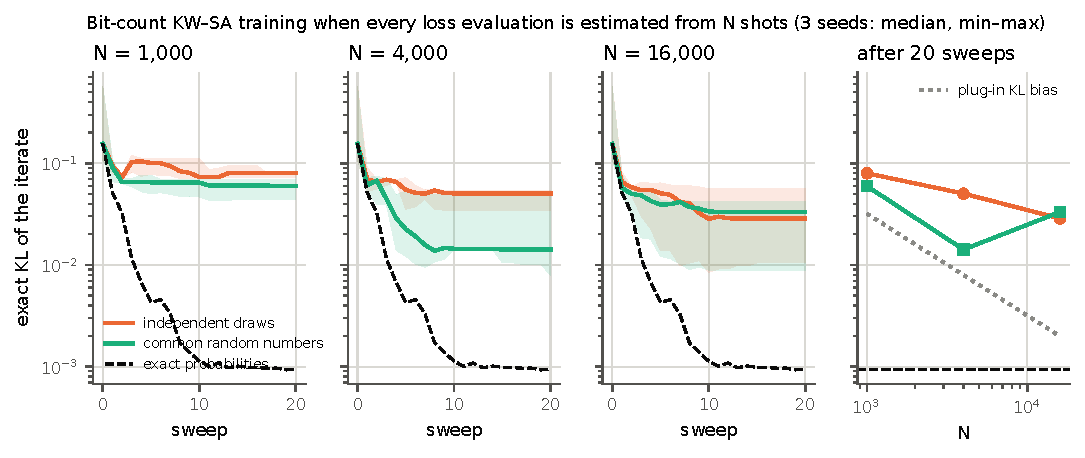
\includegraphics[width=\textwidth]{fig_bitcount_sampled_training}
\caption{Bit-count training when every loss evaluation is estimated from $N$ shots (three
seeds; median and range), with and without common random numbers, against training on exact
probabilities.  Right: the exact KL reached after 20 sweeps against $N$, with the plug-in bias
of the loss for comparison.  Run \run{bitcount\_shots/20260821T084558Z}.}
\label{fig:sampled-training}
\end{figure}

\subsection{Sequential decisions (positive result)}
\label{sec:sprt}

\paragraph{Mechanism.}
A fixed budget of $N$ shots per frame wastes most of them: a frame with $\delta = 0.3$ is decided
correctly after a dozen shots.  Wald's sequential probability ratio test \cite{wald} between the
hypotheses ``$\Pout = \tfrac12+\delta_0$'' and ``$\Pout = \tfrac12-\delta_0$'' draws shots in
blocks, after $n$ shots with $k$ ones computes the log-likelihood ratio
$\Lambda = (2k-n)\log\frac{1+2\delta_0}{1-2\delta_0}$, and stops as soon as
$\Lambda\ge\log\frac{1-\beta}{\alpha}$ (flap) or $\Lambda\le\log\frac{\beta}{1-\alpha}$ (do not
flap), up to a cap $N_{\max}$ after which the majority decides.  For a frame whose true margin
exceeds $\delta_0$ the error probability is at most about $\alpha$ ($=\beta=5\,\%$ here); for a
frame nearer the boundary than $\delta_0$ the test is slow and its error is not bounded
(\cref{fig:sprt-cost}).

\paragraph{Measurement.}
Played on the same 20 held-out games (\cref{fig:flappy-shots}, middle and right;
\cref{tab:sprt}), the sequential rule with $\delta_0 = 0.01$ and cap $10\,000$ wins \emph{every}
game at a mean of $2\,191$ shots per frame --- the fixed budget needs $10\,000$ for the same
result, $4.6\times$ more --- and with $\delta_0 = 0.005$ and cap $4\,000$ it matches the fixed
$4\,000$-shot result ($85\,\%$) at $2\,916$.  Setting $\delta_0$ at the median margin ($0.02$) fails
($30\,\%$ perfect at $820$ shots): the frames that decide a game are the near-boundary ones, and
the indifference margin must sit below \emph{their} margins (the tenth percentile, $0.004$--$0.006$),
not the typical one.  The rule needs no change to the network, no retraining, and is what one
would submit to a machine that supports mid-circuit decisions or, more simply, adaptive batch
sizes per frame.

\begin{table}[t]
\centering\small
\caption{Flappy, original controller, 20 held-out games: fixed shot budgets against the
sequential test ($\alpha=\beta=0.05$).  ``Flips'' are frames decided differently from the
exact rule.  Run \run{flappy\_shots/20260821T084601Z}.}
\label{tab:sprt}
\begin{tabular}{@{}l S[table-format=3.0] S[table-format=3.0] S[table-format=2.2] S[table-format=5.0]@{}}
\toprule
Decision rule & {perfect games (\%)} & {median pipes} & {flips (\%)} & {mean shots/frame} \\
\midrule
fixed $N = 1\,000$ & 5 & 23 & 8.36 & 1000 \\
fixed $N = 2\,000$ & 70 & 110 & 7.40 & 2000 \\
fixed $N = 4\,000$ & 85 & 110 & 6.09 & 4000 \\
fixed $N = 10\,000$ & 100 & 110 & 4.47 & 10000 \\
sequential, $\delta_0 = 0.02$, cap $10\,000$ & 30 & 88 & 7.19 & 822 \\
sequential, $\delta_0 = 0.01$, cap $4\,000$ & 80 & 110 & 6.12 & 1790 \\
sequential, $\delta_0 = 0.005$, cap $4\,000$ & 85 & 110 & 5.98 & 2916 \\
sequential, $\delta_0 = 0.01$, cap $10\,000$ & 100 & 110 & 5.06 & 2191 \\
sequential, $\delta_0 = 0.005$, cap $10\,000$ & 100 & 110 & 4.50 & 4358 \\
\bottomrule
\end{tabular}
\end{table}
